\documentclass{article}
\begin{document}
\subsection{Running examples on the MCU of the Application board}\label{ExampleOnMCU}
\subsubsection{Working principle}
The COINES SDK can be cross-compiled on PC side and downloaded into the memory of the Application board and executed there. The user can choose to download the created binary into the flash memory or into the RAM (if the binary is within the RAM memory capacity e.g., APP3.x's RAM is 256 KB).

Downloading COINES SDK example to APP3.x Flash memory will overwrite default firmware. To update the firmware again, refer to section \ref{firmwareUpdate}.

In this configuration, the COINES layer provides a simple abstraction on top of the MCU BSP (i.e. board level support layer of the microcontroller). Any \texttt{printf} command will now not output to the console, but rather to the USB connection, which appears as virtual COM port on PC side.

This mode facilitates the execution of many time-critical operations on the sensor, such as fast reading of FIFO content at high data rates.

\begin{figure}[H]
	\begin{center}
		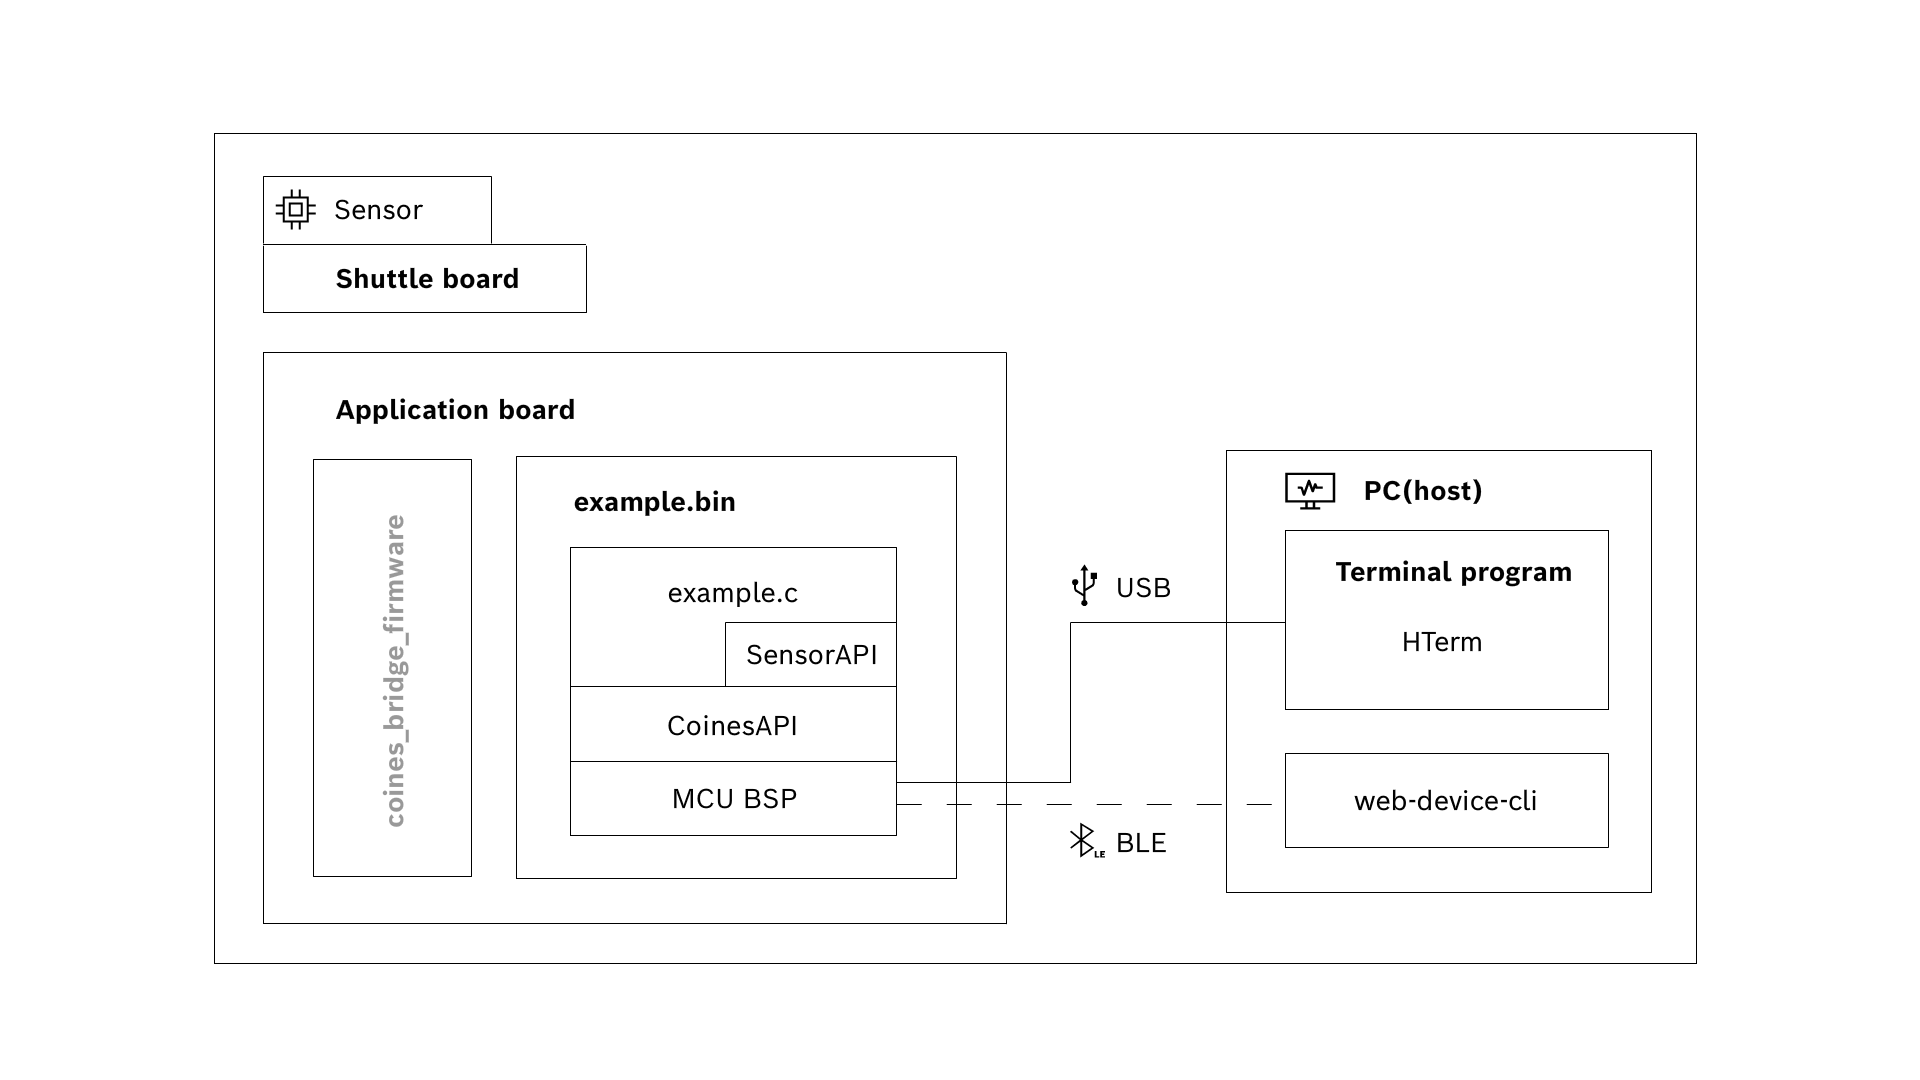
\includegraphics[width=0.9\textwidth]{coinesAPI_images/COINES_workingPrinciple_runOnMCU.png}
		\caption{Working principle: Running example on the MCU of the Application board}
	\end{center}
\end{figure}

\subsubsection{Getting started}
To get started with example execution, follow these steps:
\begin{enumerate}
	\item Make sure that \href{https://developer.arm.com/downloads/-/arm-gnu-toolchain-downloads}{GNU Embedded Toolchain for ARM} is installed on your PC and added to environmental variable \texttt{PATH}.
	\item Connect the Application board via USB, with the sensor shuttle board mounted.
	\item Open the command prompt or the terminal.
	\item Use the command \texttt{cd} to go to the directory where the example that is to be built is located.
\end{enumerate}

\subsubsection{Interfacing via BLE}
The procedure to interface via BLE involves these steps:
\begin{enumerate}
	\item Open the script to be executed (in case of SensorAPI - common.c file in the selected example folder) in your IDE
	\item Change COINES\_COMM\_INTF\_USB  to COINES\_COMM\_INTF\_BLE
	\item Change all print statments
	\begin{verbatim}
	printf(...) to fprintf(bt_w,...)
	\end{verbatim}
	\item Now follow the steps from 1 - 4 in the above section
\end{enumerate}

\subsubsection{Cross compiling}
To compile and download an example to Engineering Board's microcontroller, type any of the build commands below based on available Engineering board type and target memory location. Use '\texttt{mingw32-make}' (TDM-GCC/MinGW) or '\texttt{make}' (Linux/Cygwin/MSYS2/MacOS) for compilation.
\begin{table}[H]
	\centering
	\resizebox{\textwidth}{!}{
	\begin{tabular}{|l|l|}
		\hline
		Download example to APP2.0 MCU RAM & \texttt{mingw32-make LOCATION=RAM TARGET=MCU\_APP20 download} \\ \hline
		Download example to APP2.0 MCU FLASH & \texttt{mingw32-make LOCATION=FLASH TARGET=MCU\_APP20 download} \\ \hline
		Download example to APP3.0 MCU RAM & \texttt{mingw32-make LOCATION=RAM TARGET=MCU\_APP30 download} \\ \hline
		Download example to APP3.0 MCU FLASH & \texttt{mingw32-make LOCATION=FLASH TARGET=MCU\_APP30 download} \\ \hline
		Download example to APP3.1 MCU RAM & \texttt{mingw32-make LOCATION=RAM TARGET=MCU\_APP31 download} \\ \hline
		Download example to APP3.1 MCU FLASH & \texttt{mingw32-make LOCATION=FLASH TARGET=MCU\_APP31 download} \\ \hline
		Run an example already residing in APP2.0 Flash memory & \texttt{mingw32-make run} \\ \hline 
	\end{tabular}}
\end{table}
Note: Nicla board programs can only be executed as PC target at this moment.

\subsubsection{Viewing the results}
The ways to view the execution results are outlined as follows:
\begin{enumerate}
	\item Use a Serial Terminal application to view output.
	\begin{itemize}
		\item Windows - PuTTY, HTerm,etc.,
		\item Linux - \texttt{cat} command. Eg: \texttt{cat /dev/ttyACM0}
		\item macOS - \texttt{screen} command. Eg: \texttt{screen /dev/tty.usbmodem9F31}
	\end{itemize}
	Note: The binary on the MCU will be executed once the serial port is opened. The port must be opened including DTR signal set, otherwise the binary will not be executed. Some terminal programs such as HTerm allow explicit setting of the DTR signal.
	\item For bluetooth communication, connect the Application board to another power source and keep it within the BLE range. And use any of the below tools to view the output.
	\begin{itemize}
		\item Android app - \href{https://play.google.com/store/apps/details?id=de.kai_morich.serial_bluetooth_terminal}{Serial Bluetooth terminal}
		\item Website - \href{https://wiki.makerdiary.com/web-device-cli/}{Web Device CLI}
		\item Python script - \path{\tools\ble-nus-term\ble-nus-term.py}
	\end{itemize}
\end{enumerate}

\subsubsection{Data logging}
The user can use any serial terminal program to access and store the data provided via virtual COM port e.g HTerm has "Save output" option to store log.


\end{document}